\section{Machine Translation Engines}
In this section, we discuss about the algorithm for data extraction and the algorithm for SMT and NMT.
\subsection{Data Extraction}
The algorithm of extracting source side and language side is provided in Listing \ref{algm001}. The core of implementation is done by an AST parser we extended from the source code of Eclipse JDT \cite{032}. In this parser, we enhance the default \texttt{visit()} function which accepts an ASTNode object to a new function \texttt{visitAndExtract()}. This function behaves specifically to the MethodDeclaration node and the ASTNode objects inside this MethodDeclaration. The function for other AST objects accepts the node, the level of prefixes and the pair object. For each pairs, they contain one sequence of tokens as source and one sequence of tokens as target. Inside this function, first it will extract all tokens inside the ASTNode. Next, it will extract the prefix at n-levels for each tokens by a for loop. Final, the source and target sequence are included in the a new Pair object before adding the new object to the list. The \texttt{visitAndExtract()} function for MethodDeclaration accepts a list of pairs as input. It will create a new Pair object, visiting each ASTNode objects in the sub tree of this MethodDeclaration and extract the prefixes and related code tokens in training Github projects. 
\begin{lstlisting}[basicstyle=\small,caption={Algorithm to extract the source and target sequences by ASTParser in PrefixMap},label={algm001}]
class PrefixMapVisitor extends ASTVisitor{
    ...
	void visitAndExtract(MethodDeclaration node,int level,List<Pair> list) {
	    Pair p=new Pair();
	    node.getBody().visitAndExtract(node,level,p);
	}
	...		
	void visitAndExtract(ASTNode node,int level,Pair p) {
		String[] tokens= getTokens(node);
		
		for t in tokens{
		    String sToken=getPrefix(t,level);
		    p.getSource().append(sToken);
		    p.getTarget().append(t);
        }
	}
	...
}
\end{lstlisting}
For example in Listing \ref{example001}, the algorithm Listing \ref{algm001} will visit the \texttt{fireQueueStateChanged()} MethodDeclaration to extract information all ASTNode inside this function. The information provides us the content of varies of types of ASTNode, including the MethodInvocation, for loop and inside variables and inside MethodInvocation. The target side for each tokens is actually the code content, while the source side contains the prefix of the code tokens, which can be inputted by developers in the suggestion phase. There is a corner cases that the size of the required prefix is greater than the length of the code tokens. If that case happened, the prefix will encode the information of the whole token. For instance, the token \texttt{for} has the prefix at 9-letters as \texttt{for}. In the next section, we will discuss about important elements of MT engines we used. 

\subsection{Statistical Machine Translation for Prefix Map}
Our implementation of SMT for PrefixMap is based on a well-known toolkit Phrasal \cite{021} from StanfordNLP group. We call the source sequence as \texttt{Prefixes} and the target tokens as \texttt{Codes}. We call $prefix_{i}$ as the $i^{th}$ index prefix in the source sequence and $code_{i}$ as the $i^{th}$ index token in the target sequence. The purpose of SMT, along with NMT, is to calculate probability of each prefix is translated to target token given a context of code by different machine learning directions. For SMT, this probability contains 2 elements : the Language Model (LM) and Translation Model (TM),

\textbf{Language Model}. In SMT, the LM is calculated for the target language, means the sequence of code tokens in our problem \cite{035}.  Recently, there are newer LM models that encoded neural network as mentioned in \cite{036}. In SMT, it used the statistical language model approach called n-gram. The n-gram language model will assign probability for code sequences of the whole MethodDeclaration along with the sequence of code tokens inside the body of method. In general, the most useful purpose of LM is to calculate the probability of the last word of n-gram sequence given the previous code tokens. The LM approach is also applied in building code suggestion tool from very large code database such as \cite{031} . 

Theoretically, to predict the next code tokens, the larger number of n-gram produces the better of code token suggestion. However, large n-gram will cause exponential time increasing in the performance. In practical, Phrasal restricts the maximum size of n-gram as 7. The fastest n-gram, uni-gram, is not usually used since I provide the estimation only by the number of appearance for that code tokens.  The intuition of calculating the n-gram for code tokens is estimating the probability of the current n word given n-1 words by calculating the ratio between the number of appearance of sequence of n words per the number of appearance in sequence of n words. Smoothing is the technique that the LM are required if a word appeared in the unseen context to avoid the LM to assign zero probability. In our SMT implementation, we use the Kneser-Ney smoothing method, which is proposed by KenLM \cite{034,035,037}. We have the probabilistic model $P_{LM}$ as follow:
\noindent
\begin{equation*} 
\label{eq:001}
\begin{multlined}
 P_{LM}(code_{n}|code_{1}^{n-1}) = \\ u(code_{n}|code_{1}^{n-1})+b(code_{1}^{n-1})*P_{LM}(code_{n}|code_{2}^{n-1}))
 \end{multlined}
\end{equation*}

In this formula \ref{eq:001}, the language model probability for the $n^{th}$ code token is calculated recursively by the respected probability of the $(n)^{th}$ token given (n-2) tokens. This probability has 2 other elements for normalization, called pseudo probability \texttt{u()} and backoff metric \texttt{b} \cite{037}. The recursion will stop at the unigram distribution as follow:
\noindent
\begin{equation*} 
\label{eq:002}
\begin{multlined}
 P_{LM}(code_{n}|[]) = \\ u(code_{n}|[])+b(\epsilon)*\frac{1}{|voc of tokens|})
 \end{multlined}
\end{equation*}

In formula \ref{eq:002}, \texttt{[]} is the empty sequence. the code tokens which are unseen in data will have the probability of the second operand, since \texttt{u()} is equals to Zero.Example of how LM represented in PrefixMap in line 5 example \ref{example001} is shown in \ref{tbl001}. 

\begin{table}[]

\begin{tabular}{|l|l|l|}
\hline
\textbf{n-1 gram}                               & \textbf{nth token} & \textbf{PLM} \\ \hline
\multirow{4}{*}{for ( IQueueEnqueue listener :} & list                  & 0.82         \\ \cline{2-3} 
                                                & mListeners         & 0.78         \\ \cline{2-3} 
                                                & indices              & 0.66         \\ \cline{2-3} 
                                                & ...                & ...          \\ \hline
\end{tabular}
\caption{Example of 6-gram LM probability in Listing \ref{example001} }
\label{tbl001}
\end{table}

In this example, we see that the output of $P_{LM}$ suggests the list of variables given 5 previous tokens in the 6-gram LM. It shows the most popular popular variable as the \texttt{list} variable which is the first candidate suggested by the LM. However, the inference between source and target language also depends on another probability along with the probability of the target language. We have the second element of the SMT, the translation model.

\textbf{Translation Model}. The translation model integrates the information from LM, the mapping probability of the prefixes given the code tokens (called the phrase translation probability) and the reordering score between translated phrase and input phrase. The final output of this step provided by Phrasal is a data structure called Phrase Translation Table, which contains probability for each phrase as candidate for translation. There are three stages in producing the phrase table. The first stage is word alignment, which is done by IBM model 1 by default \cite{039}. Next, the phrase pairs of source and target languages are extracted. Final, the scoring phrase pairs process is done to assign the probability to phrase table. The probability of translation from prefixes to code tokens can be provided as follow:

\begin{equation} 
\label{eq:003}
Codes_{best}=argmax_{codes}p(Prefixes|Codes) * p_{LM}(Codes)
\end{equation}
In formula \cite{039}, the phrase translation probability \texttt{p(Prefixes|Codes)} contains information about the association between source and target tokens and the probability for reordering the phrases order between source and target language. The association between the phrase of source given the phrase of target language can be scored by relative frequency of their co-occurrence in the training set \cite{039}. There are several ways for estimating the phrase translation probability. In newest version of Phrasal, it used the Log Linear method, which calculate the translation model by this formula:

\begin{equation} 
\label{eq:003}
p(x)=exp (\sum_{i=1}^{3}\lambda _{i}*h_{i}(x))
\end{equation}

In this formula, the final translation probability will depend on the exponential of three features functions and 3 hyper parameters. They are log($\theta$) as the logarithm of  relative frequency, log(d) as the log of reorder penalty, and log($P_{LM}$) as the logarithm of language model probability. The input variable x is a random variable contains information about the candiate phrases and the position of phrases in source language.

\begin{table}[]
\begin{tabular}{|l|l|l|}
\hline
\multicolumn{1}{|c|}{\textbf{source}} & \multicolumn{1}{c|}{\textbf{target}}      & \multicolumn{1}{c|}{\textbf{p(t|s)}} \\ \hline
for ( I l : m                         & for ( IQueueEnqueue listener : mListeners & 0.88                                 \\ \hline
for ( I l : m                         & for ( Index listItem : m                  & 0.62                                 \\ \hline
\end{tabular}
\caption{Phrase table result of Line 5 Listing \ref{example001} }
\label{tbl002}
\end{table}

The translation probability extracted by the phrase table after training the data of Line 5 in Listing \ref{example001} is shown in Table \ref{tbl002}. In this table, we see that the probability for the phrase contained the sequence \texttt{f ( I l :} returns the phrase that contains the correct translation result as \texttt{mListeners}.

\textbf{Optimization of SMT for PrefixMap}. Since this corpus for PrefixMap has chracteristics of consistent length and consistent order between source and target language, we alternate the original SMT model for suit with our problem. First, we create our own alignment of source and target tokens instead of using IBM Model 1. Second, with the original output from SMT, we provide an algorithm to reverse the reordered phrases. These steps ensure the output of SMT always be consistent in length and order with the input prefixes.






\subsection{Neural Machine Translation for Prefix Map}
For NMT, we implement the solution for PrefixMap based on well-known tool Google NMT \cite{040}. The strength of NMT relies on the Encoder-Decoder architecture. As its name imply, the Encoder and Decoder layer provide an intermediate layers to convert the input sentence to a vector by an encoder model and convert from output vector to sequence of tokens in target language. These vector, called thought vector, can represent the meaning of sentence which capture other structures of sentences between source and target language. There are several details architecture of the Encode-Decoder model. Convolutional Neural Network (CNN) was proposed to learn for image processing and unsupervised learning \cite{041,042}. Graph Convolutional Network (GCN) is another architecture which can be used for graph structure data and semi-supervised classification \cite{043}. Recurrent Neural Network (RNN) is the architecture used in sequence to sequence translation \cite{044}. Long Short Term Memory (LSTM) is an improvement of RNN which help the training process to memorize the context efficiently \cite{044}. Based on characteristics of PrefixMap, we select RNN model along with LSTM as recurrent unit and Attention mechanism to apply for this problem.

\textbf{Recurrent Neural Network}. Instead of splitting the sentence as prefixes by phrases, the RNN create a sequence of vectors represented for each prefixes and provide the translated output one by one. The information about the memory of translation will be represented as a hidden state vector $h_{i}$. Compared to n-gram which is usually be limited by the length of phrase, the hidden state vector can learn the information of previous prefixes at a very long distance. RNN provides a strategy to calculate the hidden state vector at time step t based on the hidden state of previous time step by the following formula:

\begin{equation} 
\label{eq:004}
h_{t} = \sigma (W_{xh}x_{t}+W_{hh}h_{t-1})
\end{equation}
\begin{equation} 
\label{eq:005}
p_{t} = softmax(W_{hy}h_{t})
\end{equation}
In formula \ref{eq:004}, the $\sigma$ function is the non linear functions such as signmoid and tanh. The probability over the set of candidate translation at time step t will be calculated by formula \ref{eq:005}. In this formula, $x_{i}$ is an embedded vector representation for $prefix_{i}$ in the sequence of source sentence. There are 3 weight matrices that can be learned from the training. They are the recurrent weight $W_{hh}$, the feed-forward weight $W_{xh}$ and the output weight $W_{hy}$. The LSTM is selected as recurrent unit which contributes to layer of RNN.

\textbf{Attention Mechanism}. The attention model provide the better context embedding which allow to get more information from the source representation instead of used only at the initialization of hidden state. There are 2 types of attention, global attention which considers all previous prefixes and local attention which considers subset of input prefixes. In this research, we use the global attention as the information. 
The attention model creates connections between source hidden state and target hidden state. The heart of this problem is to design a context vector $c_{t}$. The new hidden state layers for target decoder can be estimated by the \texttt{tanh()} function:
\begin{equation} 
\label{eq:006}
\overline{h}^{t} =tanh(W_{c}|c_{t};h_{t})
\end{equation}

To calculate the context vector, Google NMT propose an internal vector called variable length alignment weight vector $a_{t}$ which embeds the information of both source states and target states. Given the source state s, the alignment weight vector is calculated as formula \ref{eq:007} from \cite{040}:
\begin{equation} 
\label{eq:007}
a_{t}(s)=\frac{exp(score(h_{t},\overline{h}_{s}))}{\sum (exp(score(h_{t},\overline{h}_{s^{'}})))}
\end{equation}

The score function in formula \ref{eq:007} can be calculated by dot or concatenation by vectors \cite{40}. To see how RNN and Attention work, we can look at the illustration on Listing \ref{example001}. In Figure \ref{fig:002}, the step of translation is done by following steps. First, a sequence of input prefixes will be translated to a sequence of vectors $x_{1},...,x_{k}$. In the training of RNN, $W_{xh}$ represents for the relation between input vector and the hidden source, weight $W_{hh}$ propagates the relation between different hidden vector, while $W_{hy}$ represents the weight of output vector and hidden target state. The final score for each candidate of prefix \texttt{m} are shown in \ref{fig:002}.

\begin{figure}
        \center{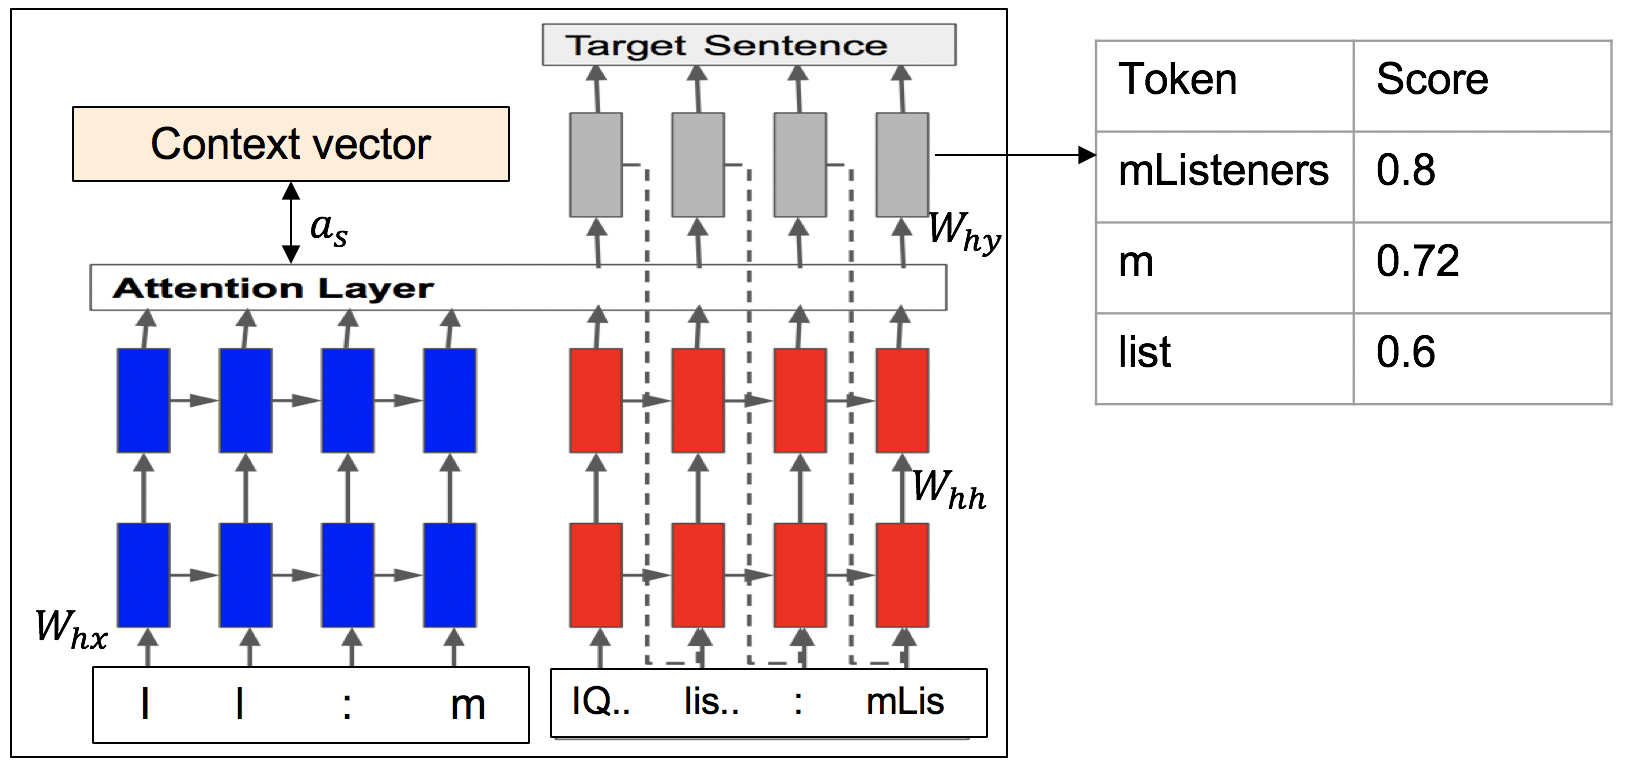
\includegraphics[width=\linewidth]
        {images/fig002.png}}
        \caption{NMT translation result of Listing \ref{example001}}
        \label{fig:002} 
\end{figure}

\textbf{Optimization of NMT for PrefixMap}. From formula \ref{eq:005}, we see that the NMT provides a distribution for all posible output, mean all possible tokens in the vocabulary. So that, it cannot work with too large vocabulary with more than 40000 words \cite{028}. To overcome this challenge, we replace the prefixes/ tokens with less than 10 times appearance as \textt{Unknown} token. We apply the same algorithm to reverse the order of the output of NMT like SMT model.  